
\section{Toy section}

This is just to test where the floating images fall in the text. Go wild and do whatever \todo[backgroundcolor=SkyBlue]{We should delete this section eventually} you want here.\\

In hac habitasse ~\cite{ref:sykepleirindeksen} platea dictumst. ~\cite{ref:JohnDoe} , Vivamus eu finibus leo. Donec malesuada dui non sagittis auctor. Aenean condimentum eros metus. Nunc tempus id velit ut tempus. Quisque fermentum, nisl sit amet  \todo{I don't like this part} consectetur ornare.

This sentence requires multiple citations to imply that it is better supported. Finally, when conducting an appeal to authority, it can be useful to cite a reference in-text, much like do quite a bit. Oh, and make sure to check out the bear in Figure \ref{bear}.

\begin{align}
	A = 
	\begin{bmatrix}
		A_{11} & A_{21} \\
		A_{21} & A_{22}
	\end{bmatrix}
\end{align}

Some random text here\\

\begin{enumerate}
	\item First numbered item in a list
	\item Second numbered item in a list
	\item Third numbered item in a list
\end{enumerate}

Pellentesque ac nisi dolor. Pellentesque maximus est arcu, eu scelerisque est rutrum vitae. Mauris ullamcorper vulputate vehicula. Praesent fermentum leo ac velit accumsan consectetur. Aliquam eleifend ex eros, ut lacinia tellus volutpat non. Pellentesque sit amet cursus diam. Maecenas elementum mattis est, in tincidunt ex pretium ac. Integer ultrices nunc rutrum, pretium sapien vitae, lobortis velit.

\begin{description}
	\item[First] This is the first item
	\item[Last] This is the last item
\end{description}

Donec nec nibh sagittis, finibus mauris quis, laoreet augue. Maecenas aliquam sem nunc, vel semper urna hendrerit nec. Pellentesque habitant morbi tristique senectus et netus et malesuada fames ac turpis egestas. Maecenas pellentesque dolor lacus, sit amet pretium \todo[backgroundcolor=Yellow, author = AM and Lars:]{Lets delete this paragraph} felis vestibulum finibus. Duis tincidunt sapien faucibus nisi vehicula tincidunt. Donec euismod suscipit ligula a tempor. Aenean a nulla sit amet magna ullamcorper condimentum. Fusce eu velit vitae libero varius condimentum at sed dui.

\begin{figure}
	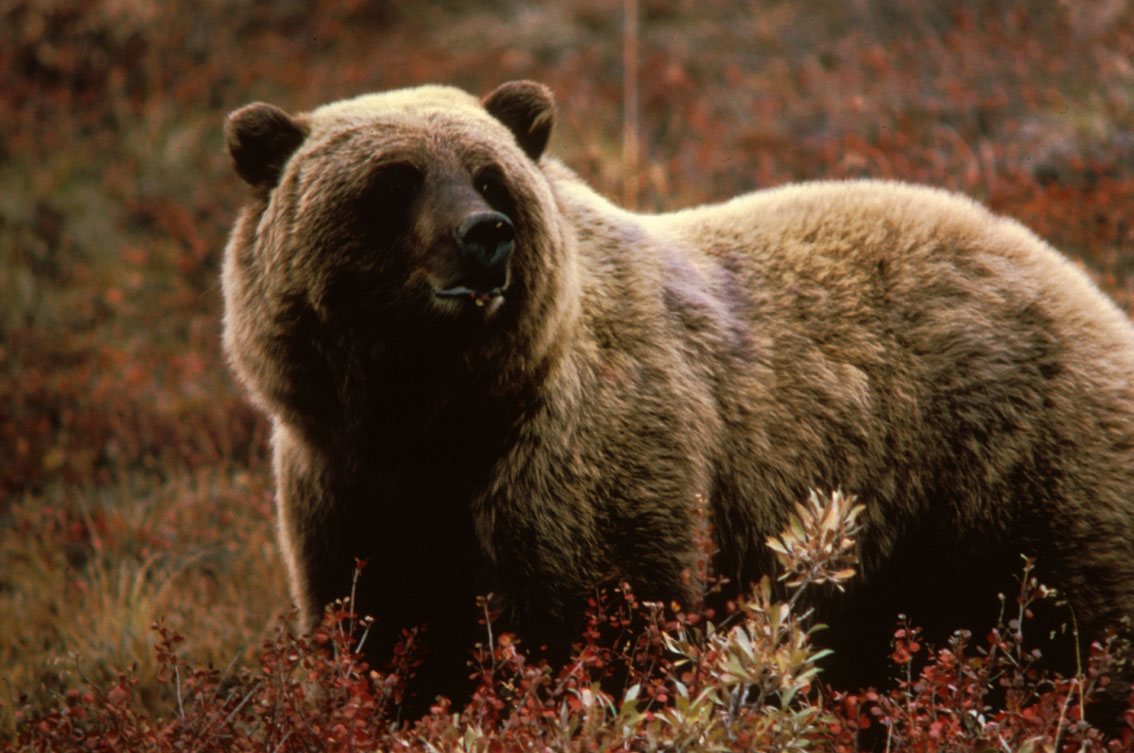
\includegraphics[width=\linewidth]{bear.jpg} % Figure image
	\caption{A majestic grizzly bear} % Figure caption
	\label{bear} % Label for referencing with \ref{bear}
\end{figure}

Aliquam elementum nulla at arcu finibus aliquet. Praesent congue ultrices nisl pretium posuere. Nunc vel nulla hendrerit, ultrices justo ut, ultrices sapien.  \todo[backgroundcolor=Fuchsia, author = This Person say:]{Maybe this can go to page 4} Duis ut arcu at nunc pellentesque consectetur. Vestibulum eget nisl porta, ultricies orci eget.

\begin{table}
	\caption{Example table}
	\centering
	\begin{tabular}{llr}
		\toprule
		\multicolumn{2}{c}{Name} \\
		\cmidrule(r){1-2}
		First Name & Last Name & Grade \\
		\midrule
		John & Doe & $7.5$ \\
		Richard & Miles & $5$ \\
		\bottomrule
	\end{tabular}
\end{table}
